\chapter{Backend}

Bevor wir zur Besprechung der Umsetzung des eigentlichen Backends übergehen, wollen wir zuerst einige grundsätzliche Überlegungen zur Art des Prozesses, den wir für unser Backend einsetzen wollen, festhalten.

\section{Art des Prozesses}\label{lbl_prozess_art}

\subsection{Prozesse unter Android}

Da in der Entwicklung für das Android-Betriebssystem ein etwas erweitertes Vokabular für die Beschreibung des Applikations-Lebenszyklus verwendet wird, wollen wir zuerst kurz auf einige dieser Begriffe im Android-Kontext eingehen.

Applikationen laufen unter Android grundsätzlich in einem eigenen Thread den das Betriebssystem als separaten Linux-Prozess startet und werden auch vom Betriebssystem wieder beendet. Sollen Komponenten in einem eigenen Prozess laufen, können weitere Threads gestartet werden\cite{adglc}. Diese können über die standard Thread-Objekte von Java erzeugt werden, werden aber mit dem Applikations-Prozess terminiert, sollte Android entscheiden dass dieser nicht mehr benötigt wird. Um dies, wenn Ressourcen benötigt werden sollten, möglich effizient durchzuführen, werden Prozesse vom Betriebssystem einfach abgewürgt (ein kill-Signal wird gesendet) und keinerlei Aufräumfunktionen werden ausgeführt. Applikationen sind daher selbst dafür verantwortlich, ihren Status zu sichern, wenn sie in den Hintergrund geschickt werden\cite{adbmt}.

Unser Erkennungs-Backend sollte nun aber auch unabhängig vom Frontend weiterlaufen. Grundsätzlich wäre das beenden des Backend-Threads beim Schliessen des Frontends kein grösseres Problem, da wir davon ausgehen können, dass eventuell erst nach Beendung des Frontend-Threads eintreffende Resultate für den Benutzer nicht mehr relevant sind und verworfen werden können bzw. nicht mehr fertig gerechnet werden müssen. Allerdings wäre es zu bevorzugen, wenn bei einem erneuten Aufruf des Frontends der Backend-Thread schon im Speicher vorhanden ist und nicht noch neu initialisiert werden muss. Die Initialisierung des Backends kann je nach verwendeter Erkennungs-Methodik recht aufwendig sein. So muss etwa bei der Graphen-Methode zuerst die XML-Datei, in welcher der Graph gespeichert ist, eingelesen und der Graph aufgebaut werden. Der Benutzer erwartet möglichst schnell mit der Eingabe beginnen zu können und eine Initialisierung bei jeder Versuch dazu sollte ihm daher nicht zugemutet werden.

Neben den normalen Threads aus Java kennt Android noch spezialisierte Prozesse, die unabhängig von der Ursprungs-Applikation weiterlaufen können. Für uns interessant sind hier vor allem die Services und die Broadcast-Receiver.

\subsubsection{Broadcast-Receiver}

Broadcast-Receiver werden hauptsächlich dazu verwendet, im Hintergrund auf Ereignisse zu reagieren. Die Handhabung diese Ereignisses durch den Receiver muss innerhalb einer gegebenen Zeit erfolgen\footnote{Im Moment beträgt die zur Verfügung stehende Zeit 10 Sekunden, danach kann der Prozess jederzeit abgewürgt werden\cite{adbmt}}, wodurch diese nur im Speicher gehalten werden müssen, wenn ein solches Ereignis eintrifft. Broadcast-Receiver sind daher also gut geeignet um kurze Arbeiten als Reaktion auf eine externen Stimulus durchzuführen und werden etwa benutzt um auf Alarme oder Positions-Änderungen zu reagieren. Da sie aber nach Beendigung ihrer Aufgabe voraussichtlich wieder terminiert werden, würden sie für unseren Backend-Prozess keinen Vorteil darstellen, da sich die Frage der Reinitialisierung ebenfalls wieder stellen würde.

\subsubsection{Services}

Services sind unter Android sehr vielseitig und durch sie können Applikationen langlaufende Operationen im Hintergrund ausführen. Grundsätzlich ist ihre Laufzeit nicht beschränkt und ihr Verhalten in dieser Zeit wird weitestgehend von der Applikation bestimmt. So können sie etwa vom restlichen Programm unabhängige Operationen ausführen, auf gemeinsame Singelton-Objekte zugreifen oder gar in einen eigenen Prozess ausgelagert werden.

Services können allerdings vom Betriebssystem jederzeit abgeschossen werden, wenn es Ressourcen benötigen sollte. Allerdings wird sich Android merken, wenn es Services, die weiter laufen wollen, terminiert. Wenn wieder genug Arbeitsspeicher verfügbar ist, werden die beendeten Services wieder neu gestartet. Auch ist es möglich, dass Services beantragen, als Vordergrund-Prozesse behandelt zu werden und so recht gut vor dem Terminieren geschützt sind. Dies muss dem Benutzer allerdings angezeigt werden, damit sich dieser des laufenden Prozesses bewusst ist.

Für unser Backend sollte ein Service also die am besten geeignete Prozess-Form sein, da wir den Backend-Service im Hintergrund weiter laufen lassen können, nachdem eine Eingabe getätigt wurde. Eine Terminierung bei zu wenig vorhandenem Speicher können wir akzeptieren, da der Service danach wieder neu gestartet werden sollte und die Initialisierung vom Benutzer unbemerkt im Hintergrund stattfinden kann. Wir benötigen daher auch nicht die Privilegien eines Vordergrund-Prozesses.
%================================================

\section{Analyse}

\subsection{Initialisierung}

\subsection{Ablauf der Erkennungs}

Um den Ablauf der Erkennung möglichst flexibel zu machen, wurde dieser in mehrere Phasen aufgeteilt. Einige dieser Phasen sollen wiederum in mehrere Einzelschritte aufgeteilt werden.

\begin{figure}[h]
   \centering
   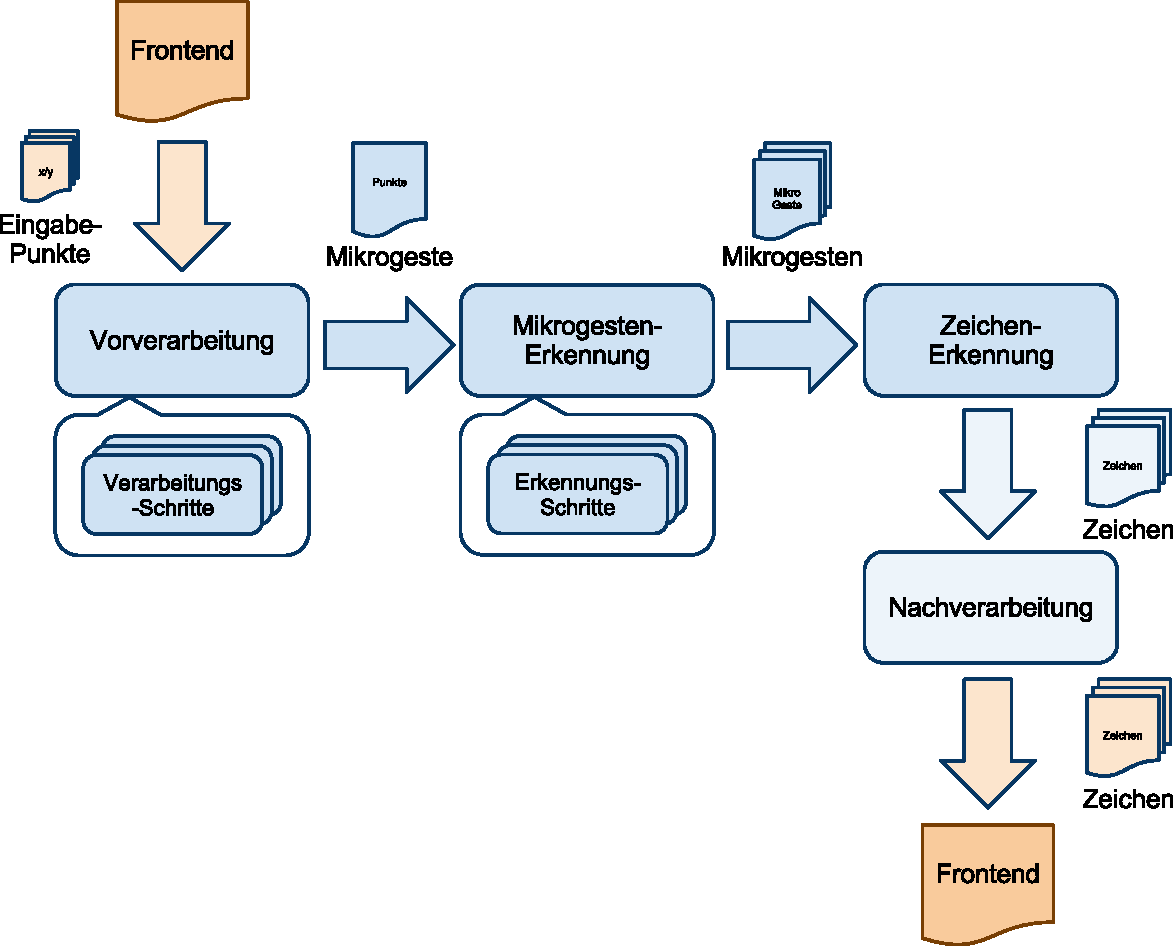
\includegraphics[width=\textwidth]{img/erkennungs_ablauf.pdf} 
   \caption{Erkennungs-Ablauf}
   \label{fig:erkennungs_ablauf}
\end{figure}

Zuerst soll eine Vorverarbeitung der Eingabe-Punkte durchgeführt werden, in der etwa eine Normierung, eine Glättung, eine Filterung oder ähnliches dieser durchgeführt werden kann. Diese Verarbeitungs-Schritte sollen sich nicht gegenseitig ausschliessen, sollen aber auch optional sein, da einige der dazu möglichen Algorithmen sehr rechenaufwendig sind.

Die zweite Phase soll die Erkennung der Mikrogesten sein. Auf diese soll in mehrere Erkennungs-Schritte aufgeteilt sein, die gegebenenfalls auch deaktiviert werden können.

Als nächstes soll die Zeichen-Erkennung durchgeführt werden. Diese soll allerdings in sich geschlossen funktionieren und nicht zwingend weiter in Teil-Schritte aufgeteilt werden. Das Erkennungs-Verfahren als ganzes soll allerdings austauschbar sein.

Die vierte und letzte Phase soll die Nachverarbeitung der erkannten Zeichen sein. Dies kann etwa bedeuten, das gewisse Zeichen wieder verworfen werden oder das die Gewichtung der Erkennungs-Wahrscheinlichkeit der Zeichen angepasst wird.

\subsubsection{Vorverarbeitung}

Häufig könnte die Erkennungsgenauigkeit der Mikrogesten-Erkennung durch eine passende Vorverarbeitung der Eingabe-Punkte erheblich verbessert werden. Allerdings sind viele der geeigneten Algorithmen sehr rechenaufwendig und können die Geschwindigkeit der Erkennung selbst auf leistungsfähigen Systemen erheblich verlangsamen\footnote{Unsere Test-Hardware, das Nexus One von Google mit einem 1 GHz Snapdragon Prozessor, benötigte bei einigen Algorithmen etwa mehrere Sekunden für die Glättung der Eingabe-Punkte normaler Buchstaben}. Daher war es unser Ziel, den Einsatz solche Vorverarbeitungs-Algorithmen zwar zu ermöglichen, diese allerdings optional zu machen. Insbesondere soll es möglich machen, dass diese in einer späteren Version auch aus dem Frontend heraus zu aktivieren oder deaktivieren.

Auch wollten wir eine serielle Abarbeitung von mehreren Vorverarbeitungs-Schritten möglich zu machen. Dabei muss es möglich sein, diese in einer festlegbaren Reihenfolge ausgeführt werden. So könnte zum Beispiel gewünscht werden, dass zuerst gewisse Punkte heraus gefiltert werden, bevor eine Glättung durchgeführt wird, um den Rechenaufwand für diese zu reduzieren.

\subsubsection{Mikrogesten-Erkennung}

Auch bei der Erkennung der Mikrogesten soll es möglich sein, diese in mehrere Schritte aufzuteilen und diese in einer definierbaren Reihenfolge durchzuführen. Dies kann etwa zum Testen verschiedener Ansätze nützlich sein, aber auch zum Feintuning eines speziellen Ansatzes. Ein Beispiel wäre hierbei, dass zuerst die harten Kanten im Pfad der Eingabe-Punkte detektiert werden und danach die einzelnen Mikrogesten in diesen Kanten gesucht werden.

Auch hier soll eine Anpassung zur Laufzeit durch das Frontend grundsätzlich möglich sein und von unserem Design unterstützt werden.

\subsubsection{Zeichen-Erkennung}

Auch das Austauschen des Algorithmus zur Zeichen-Erkennung zur Laufzeit soll grundsätzlich möglich sein. Allerdings soll es nur möglich sein, diesen als Ganzes auszutauschen. Eine Unterteilung in Teilschritte soll nicht von der Architektur her vorgeschrieben werden und eine Umorganisation dieser während der Laufzeit ist nicht angedacht, da wir die eigentliche Zeichen-Erkennung als monolithischen Vorgang gestalten wollen.

So können verschiedene Ansätze zur Zeichen-Erkennung anhand der Mikrogesten miteinander verglichen und alternative Erkennungs-Strategien angeboten werden. Neben dem in dieser Arbeit verwendeten Ansatz für eine Erkennung durch einen Graphen, ist etwa eine Erkennung über ein neurales Netz eine naheliegende Möglichkeit.

Speziell für eine Erkennungs-Ansatz über ein neurales Netz, aber auch für den Graphen-Ansatz, wäre eine Möglichkeit zur Anpassung der zur Erkennung verwendeten Datenbasis von Vorteil. Daher wollen wir auch eine Möglichkeit zur Nachverarbeitung der Daten bieten.

\subsubsection{Nachverarbeitung}

Für die Nachverarbeitung wollen wir einen zur Zeichen-Erkennung analogen Ansatz verwenden. Das heisst dass es möglich sein soll, den verwendete Algorithmus auszutauschen, eine Unterteilung in Teilschritte soll aber nicht gefordert werden. Im Gegensatz zur Zeichen-Erkennung soll die Nachverarbeitung aber optional sein.

Mögliche Einsatz-Zwecke für Nachverarbeitungs-Algorithmen wäre etwa, wie bereits erwähnt, die Anpassung der vorhandenen Datenbasis an den individuellen Benutzer in einem Trainingsmodus, die weitere Einschränkung oder Anpassung der Erkennungs-Wahrscheinlichkeiten der erkannten Zeichen, etwa anhand eines Wörterbuches.
%================================================

\section{Design}

\subsection{Schnittstellen}

Wie bereits in \ref{lbl_prozess_art} besprochen, wollen wir für das Backend einen Service definieren. Damit dieser auch wirklich unabhängig (also in einem eigenen Prozess) vom Frontend läuft, soll dieser ein Remote-Service sein. Dies bedeutet, dass wir für die Kommunikation zwischen dem Frontend und dem Backend Schnittstellen definieren müssen, um die Inter-Prozess-Kommunikation abzuwickeln. Android stellt dafür eine eigenen Dialekt der Interface Definition Language bereit, der sich wenig überraschend "Android Interface Definition Language" (kurz AIDL) nennt.

Die Schnittstellen, die wir benötigen werden, lassen sich in zwei Gruppen unterteilen: Die eigentliche Zeichen-Erkennung und die Verwaltung der Erkennungs-Algorithmen.

\subsubsection{Zeichen-Erkennung}

Die Schnittstellen für die Zeichen-Erkennung sind relativ simpel und direkt: Es müssen Eingabe-Punkte an das Backend gesendet werden und es müssen die erkannten Zeichen an das Frontend zurück gegeben werden.

\begin{lstlisting} [caption={Schnittstellen für die Zeichen-Erkennung},label=intrf_detection]
interface IDetectionService {
    /**
     * Registering callback interface with service.
     */
    void registerCallback(
		IReturnRecognisedCharacters cb);
    
    /**
     * Remove a previously registered callback interface.
     */
    void unregisterCallback(
		IReturnRecognisedCharacters cb);
    
    /**
     * Add TouchPoints to detection queue
     */
    void addTouchPoints(in List<TouchPoint> points);
}

oneway interface IReturnRecognisedCharacters {
    /**
     * Return recognised Characters
     */
    void recognisedCharacters(
		out List<Character> characters);
}
\end{lstlisting}

\subsubsection{Verwaltung der Erkennungs-Algorithmen}

\subsection{Erkennungs-Alogrithmen}

(Klassendiagramm, Sequenzdiagramm)
%================================================

\section{Implementation}

(...)
%================================================

